\documentclass[11pt, oneside]{article} 
\usepackage{geometry}
\geometry{letterpaper} 
\usepackage{graphicx}
	
\usepackage{amssymb}
\usepackage{amsmath}
\usepackage{parskip}
\usepackage{color}
\usepackage{hyperref}

\graphicspath{{/Users/telliott_admin/Dropbox/Tex/png/}}
% \begin{center} 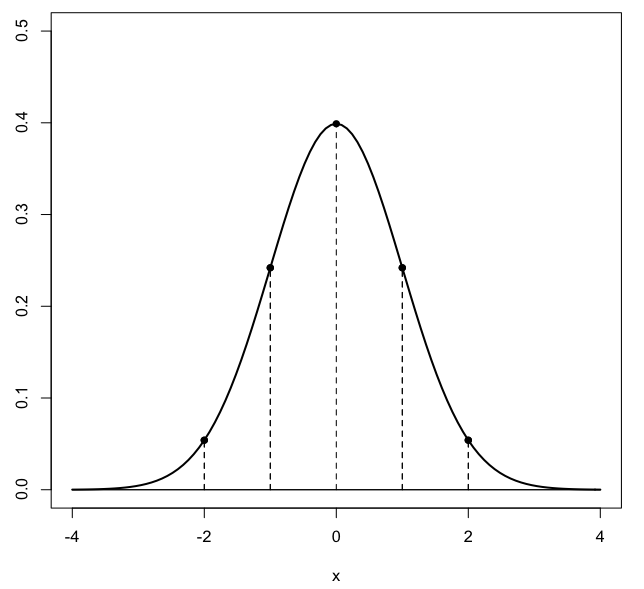
\includegraphics [scale=0.4] {gauss3.png} \end{center}

\title{Basic geometry and congruence of triangles}
\date{}

\begin{document}
\maketitle
\Large

\subsection*{Euclid and the postulates}
Greek geometry starts hundreds of years before Euclid, whose life overlapped (on both ends) that of Alexander the Great.  Euclid died about 270 BC, although his life and death are shrouded in mystery. 

Euclid's book \emph{Elements} is still an excellent place to begin surveying the foundations of geometry.

Euclid's geometry is mainly constructions (geometric figures) drawn with a pencil on a flat piece of paper, using a straight-edge or a compass or both.  

\begin{center} 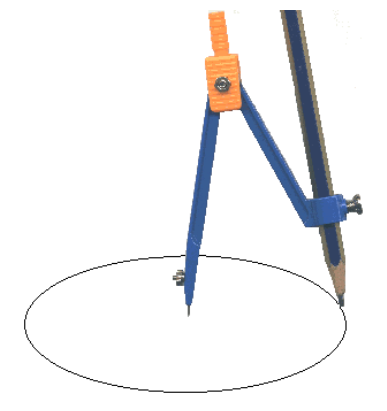
\includegraphics [scale=0.3] {compass.png} \end{center}

Here are Euclid's first three postulates --- statements that are assumed to be true:

$\circ$  A straight line segment can be drawn joining any two points.

$\circ$   Any straight line segment can be extended indefinitely in a straight line.

$\circ$   Given any straight line segment, a circle can be drawn having the segment as radius and one endpoint as center.

Let us assume these as well.

We finesse the difficulty in defining what is meant by \emph{straight} in the real world.  If you've ever done any carpentry, for example, you probably know that unknown edges are determined to be straight by comparison with known straight edges.  But the mental construct of  "a straight line is the shortest distance between two points" gets around this limitation.

The fourth postulate is:

$\circ$   All right angles are congruent, that is, equal to each other.

This one prompts a different question:  what is a "right angle"?  

If a line segment is drawn with one end on a line, let us refer to the two angles the line segment forms with the line as adjacent angles.

The definition of a right angle is this:  if these two adjacent angles are equal, then they are both right angles.

\begin{center} 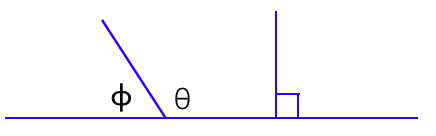
\includegraphics [scale=0.4] {perps.png} \end{center}

On the left, one of the angles, $\phi$, is smaller than the other one, $\theta$.  

Alternatively, on the right, the two angles have equal measures.  In this case we can conclude that both angles are right angles.   A right angle is frequently designated by drawing a small square at the intersection. Since both angles are right angles, only one square is needed or usually drawn.

In all cases, the sum of the two angles $\phi + \theta$ is equal to two right angles or 180 degrees.  There is nothing particularly special about $180$ degrees for two right angles or $360$ degrees for one whole turn.  

Well, there is one thing:  there are \emph{approximately} 360 days in a year, which marks the sun's track across the sky.  In his book, \emph{Measurement}, Lockhart adopts the convention that one whole turn is equal to $1$.  

Later, we'll see that one whole turn is defined as $2 \pi$ radians, and that convention turns out to be quite important.

Now, extend those lines below the horizontal

\begin{center} 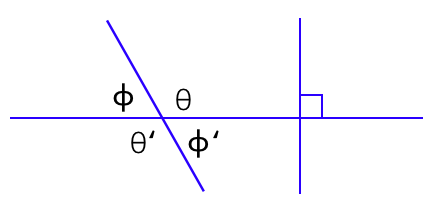
\includegraphics [scale=0.4] {perps2.png} \end{center}

We said that the sum of the two angles $\phi + \theta$ is equal to two right angles, but so is the sum $\theta + \phi'$, for the same reason.

\[ \phi + \theta = \theta + \phi' \]
We conclude that $\phi = \phi'$ and $\theta = \theta'$.  On the right, if any one of the angles where two lines cross is a right angle, then all four are right angles.

This is called the vertical angle theorem.

There is a simple method to construct a line segment perpendicular to a line at a particular (given) point, or alternatively, through any point not on the line (see the video at the url):

\url{https://www.mathopenref.com/constperpextpoint.html}

\subsection*{parallel postulate}

All this seems rather obvious.  

The fifth and final postulate is more subtle:

$\circ$   If two lines are drawn which intersect a third in such a way that the sum of the inner angles on one side is less than two right angles, then the two lines inevitably must intersect each other on that side if extended far enough.
\begin{center} 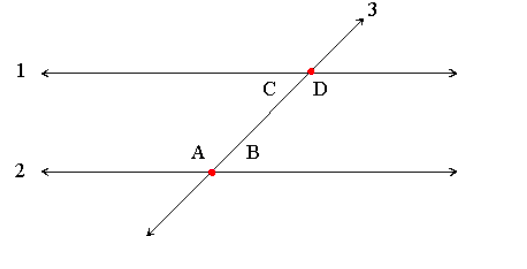
\includegraphics [scale=0.5] {alternate_interior_angles.png} \end{center}

Line $1$ and line $2$ are parallel, if and only if, $A + C = B + D = 180 = 2$ right angles.  This postulate is equivalent to what is known as the parallel postulate.

\url{http://mathworld.wolfram.com/EuclidsPostulates.html}

Consider a familiar situation where this is not true.  Suppose we are doing geometry on the surface of a sphere, such as the earth.  Two adjacent lines of longitude can be drawn so as to cross the equator at right angles, and the lines are parallel there, but they meet (intersect) at the poles.  

The parallel postulate only holds for geometry on a \emph{flat} surface.

\subsection*{axioms}

Euclid also lists five axioms.  Here are two examples:

$\circ$   Things that are equal to the same thing are also equal to one another.

$\circ$   If equals are added to equals, then the wholes are equal.

We will see how to proceed from the postulates and axioms to various proofs.  \emph{Given these assumptions}, we can prove theorems that must be true.

\subsection*{Thales}
I'm a big fan of William Dunham's books --- three of them are listed in the References.  

Dunham has written a lot about the history of mathematics in Greece, starting with Thales (624-546 BC), who was from a Greek town called Miletus on the coast of Asia Minor (modern Turkey).  He lived long before Euclid.  Although none of his writing survives, it is believed that Thales proved several early theorems including one we saw above

$\circ$  The vertical angles formed by two straight lines crossing, are equal.
\begin{center} 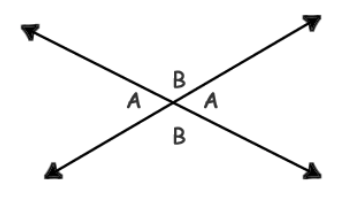
\includegraphics [scale=0.4] {vertical_angles.png} \end{center}
This theorem depends on a property of straight lines.  In the proof, we used the axiom  "equals added to equals are equal", alternatively "equals subtracted from equals are equal."

$\circ$  The angle sum of a triangle is equal to two right angles.
\begin{center} 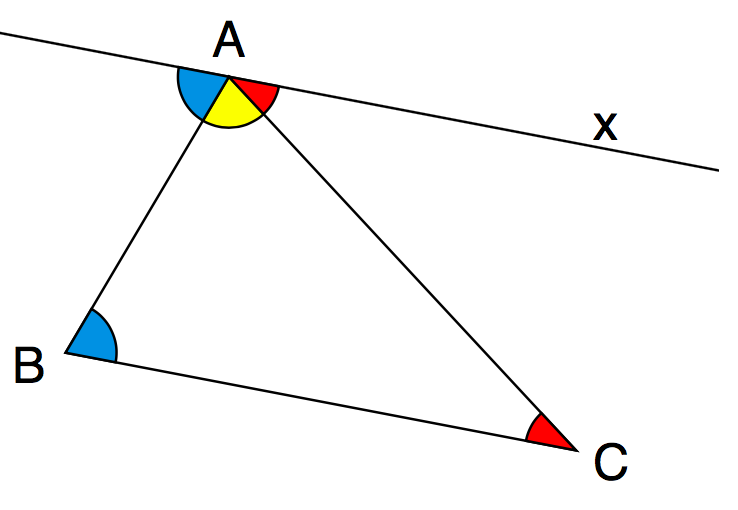
\includegraphics [scale=0.3] {triangle_sum_angles.png} \end{center}

This theorem depends in turn on a theorem which we laid the groundwork for above but did not state explicitly.

In the figure below, if $1$ is parallel to $2$, we said that $A + C = B + D = 180$ degrees.  \begin{center} 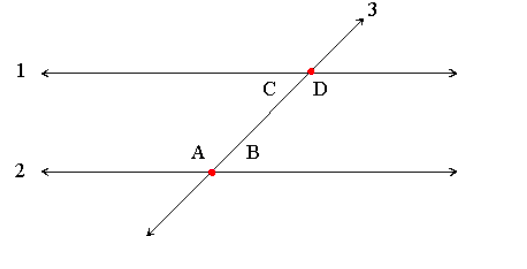
\includegraphics [scale=0.5] {alternate_interior_angles.png} \end{center}

But we also know from the properties of two lines given above that $A + B = 180$ degrees. So
\[ A + C = 180 = A + B \]
and then
\[ C = B \]

This is called the theorem on alternate interior angles.  Given this, you can go back to the angles of a triangle problem and follow the colors to the proof.

\subsection*{another proof}
Here is an alternative proof of the theorem on the sum of angles in a triangle adding to 180 degrees..

Imagine walking around the perimeter of a triangle in the counter-clockwise direction.  At each vertex we turn left by a certain number of degrees, $t$, called the exterior angle.  After passing through all three vertices, we must end up facing in the same direction as we started.

\begin{center} 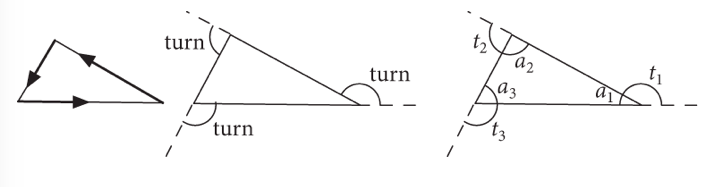
\includegraphics [scale=0.5] {triangle_sum_angles2.png} \end{center}

\[ t_1 + t_2 + t_3 = 360 \]

In addition, for each vertex, the interior angle $a_i$ plus the exterior angle $t_i$ add up to $180$ degrees.  If we add up all three pairs, we obtain
\[ (t_1 + a_1) + (t_2 + a_2) + (t_3 + a_3) = 3 \cdot 180 = 540 \]
By subtraction
\[ a_1 + a_2 + a_3 = 180 \]

\end{document}